% software-applications-ai-search-michaelmas-2011-summative.tex -- Summative report
%
% This is a solution of the summative assignment of the AI Search submodule of
% the Software Applications module held at the Durham University, Durham,
% United Kingdom.  Michælmas term 2011.
%
% Based on \cite{minarcsys}, \cite{minarip} and \cite{minarcsysdb}
%
% Copyright © 2008–2011 Jan Minář <rdancer@rdancer.org>
%
% This work is free software; you can redistribute it and/or modify
% it under the terms of the GNU General Public License version 2 (two),
% as published by the Free Software Foundation.
%
% This work is distributed in the hope that it will be useful,
% but WITHOUT ANY WARRANTY; without even the implied warranty of
% MERCHANTABILITY or FITNESS FOR A PARTICULAR PURPOSE.  See the
% GNU General Public License for more details.
%
% You should have received a copy of the GNU General Public License along
% with this work; if not, write to the Free Software Foundation, Inc.,
% 51 Franklin Street, Fifth Floor, Boston, MA 02110-1301 USA.

\documentclass[10pt,twocolumn]{article}


\usepackage[utf8]{inputenc}
\pdfoutput=1
\usepackage[pdftex]{graphicx}     
\usepackage{amssymb}    
\usepackage{harvard}
\usepackage{url}
\usepackage{fancyhdr}
\usepackage{lastpage}
\usepackage{rotating}  % \begin{sideways}

\pagestyle{fancy}
\fancyhead{}
%\chead{Computer Systems --- Summative Assignment}
%\chead{Copyright © 2008–2010 Jan Minář {\tt <rdancer@rdancer.org>}}
	%\\ page \thepage\ of \pageref{LastPage}}

\chead{ \small \sc
    Travelling Salesman Problem --- Software Applications (AI Search)
}
\cfoot{ \small \sc
    Copyright © 2011 Jan Minář {\tt <rdancer@rdancer.org>}
	\\ \thepage
}

\author{Jan Minář {\tt <rdancer@rdancer.org>}}
%\date{December 1, 2010}

%%%%%%%%%%%%%%%%%%%%%%%%%%%%%%%%%%%%%%%%%%%%%%%%%%%%%%%%%%%%%%%%%%%%%%%%%%%%%%
% ``Title''
%	-- the assignment

% No LaTeX command to make a subtitle, but possible using custom code (not
% including due to absence of license, but it is possible):
% <http://groups.google.com/group/comp.text.tex/msg/3aa4f67d8b3a979b?hl=en-EN&pli=1>
\title{Travelling Salesman Problem}

\begin{document}
\bibliographystyle{agsm}
\setcounter{section}{-1}  % Start section numbering from zero

\maketitle

% Note: This is a ‘report’


\section{Abstract}
\thispagestyle{fancy}

In this report,\footnote{This is a summative assignment in the Software Applications (Artificial Intelligence Search) sub-module taught at Durham University, UK in Michælmas 2010.}

% Note: use \begin{sidewaysfigure} for a landscape figure with proper captioning
\begin{figure}

    % Reduce margins -- solution from
    % http://stackoverflow.com/questions/857483/custom-margin-settings-for-figure-in-latex
    % accessed on 2010-12-07
    %\noindent
    %\makebox[0.3\textwidth]{
	%\fbox{
	    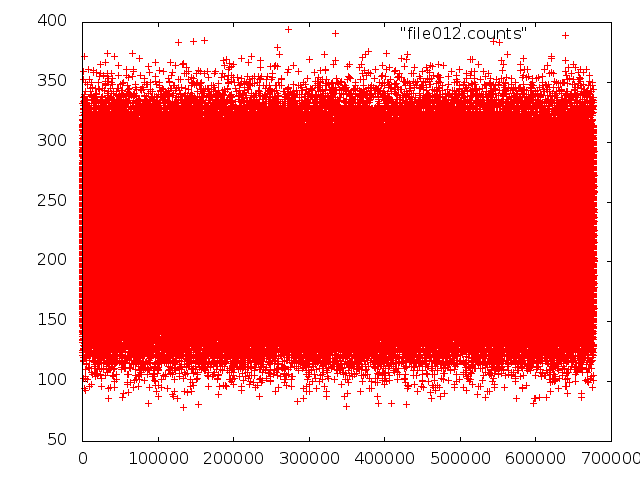
\includegraphics[width=0.3\paperwidth]{file012.png}
	%}
    %}

    \caption{
	12 cities --- some graph
    }
    \label{file012}
\end{figure}


%\renewcommand\bibname{Bibliography and Data Sources}

% Have the references on a new page
\pagebreak

\nocite{Russell2003}

\bibliography{references}
\thispagestyle{fancy}

\end{document}
